
\subsection{Software Commands and Version Numbers}
We provide the detailed commands for the various analyses we performed.
\begin{itemize}
\item

RAxML v8.2.6 was used to estimate gene trees on the phylogenomic simulated data with arguments ``-m GTRGAMMA -p 12345 -n  $<$jobname$>$  -s  $<$input$>$''.
\item
RAxML v8.2.6 was used to run MRL with arguments ``-m BINGAMMA -p 12345 -n $<$jobname$>$ -s $<$input$>$''.
\item Mrpmatrix (available from \url{https://github.com/smirarab/mrpmatrix}) was used to calculate the matrix for MRL.
\item
ASTRAL v4.7.8 was passed to FastRFS and ASTRAL-SIESTA to calculate the search space.
\item
BCD v1.0.1 was used to calculate BCD trees using arguments ``--filetype newick''
\item
FastRFS v2.0 was used with and without SIESTA, with arguments
``--count'', ``--greedy'', ``--majority'', ``--strict'', and
``--single'' used as necessary to count the number of optimal trees,
output consensus trees, or output a single optimal tree. The ``-e''
option was used to pass it additional trees. 
\item
ASTRID v1.1 was used to calculate trees for  the constraint set of FastRFS-enhanced, using no additional options.
\item

Dendropy v4.0.3 was used to calculate error rates with the function

\begin{verbatim} dendropy.calculate.treecompare.false_positives_and_negatives\end{verbatim}

\end{itemize}


\clearpage

\subsection{Additional Figures and Tables}

%\subsection{Numbers of optimal trees}


\begin{table}[h]
\centering

\begin{tabular}{|rrr|lll|}
 
\hline
 & & & astral & fastrfs-basic & fastrfs-enh\\
taxa&ngenes&scaffold&&&\\


\hline 
\hline
100&6&20\%	&$9.36$	&$3.52\times 10^{2}$	&$1.21\times 10^{3}$\\
100&6&50\%	&$4.00$	&$1.31\times 10^{2}$	&$1.71\times 10^{3}$\\
100&6&75\%	&$1.72$	&$7.27\times 10^{1}$	&$1.57\times 10^{2}$\\
100&6&100\%	&$1.04$	&$2.49\times 10^{1}$	&$3.40\times 10^{1}$\\
\hline
500&16&20\%	&$1.62\times 10^{3}$	&$6.09\times 10^{7}$	&$1.96\times 10^{9}$\\
500&16&50\%	&$3.94\times 10^{1}$	&$1.97\times 10^{8}$	&$7.62\times 10^{8}$\\
500&16&75\%	&$4.23\times 10^{1}$	&$1.37\times 10^{8}$	&$6.99\times 10^{8}$\\
500&16&100\%	&$1.00$	&$5.36\times 10^{6}$	&$2.93\times 10^{7}$\\
\hline
1000&26&20\%	&$6.48\times 10^{5}$	&$2.32\times 10^{15}$	&$2.50\times 10^{16}$\\
1000&26&50\%	&$3.60\times 10^{4}$	&$9.17\times 10^{14}$	&$1.11\times 10^{18}$\\
1000&26&75\%	&$5.67\times 10^{2}$	&$2.51\times 10^{14}$	&$1.68\times 10^{17}$\\
1000&26&100\%	&$1.00$	&$1.97\times 10^{13}$	&$5.03\times 10^{13}$\\
\hline
\end{tabular}

\caption[Number of FastRFS optimal trees for simulated
  unrooted supertree datasets.]{Number of FastRFS optimal trees for simulated
  unrooted supertree datasets. We show the mean number
  of optimal trees averaged over 25 replicates for 100 and 500 taxa,
  and 10 replicates for 1000 taxa.} \label{tab:supertree_counts}
\end{table}

\begin{table}
\centering
\begin{tabular}{|rr|r|}
 
\hline
 & & astral\\
ILS&ngenes&\\


\hline 
\hline
Moderate ILS&5&	$2.12$\\
Moderate ILS&10	&$1.12$\\
Moderate ILS&25	&$1.04$\\
\hline
High ILS&5&	$1.64$\\
High ILS&10&	$1.00$\\
High ILS&25&	$1.00$\\
\hline
Very High ILS&5	&$1.20$\\
Very High ILS&10	&$1.08$\\
Very High ILS&25	&$1.04$\\
\hline
\end{tabular}

\caption[Number of ASTRAL optimal trees for simulated
  50-taxon phylogenomic datasets where all gene trees are complete (i.e., no missing data)]{Number of ASTRAL optimal trees for simulated
  50-taxon phylogenomic datasets where all gene trees are complete (i.e., no missing data). We show the mean number
  of optimal trees averaged over 25 replicates} \label{astral_counts}
\end{table}


\begin{table}
\centering

\begin{tabular}{|rr|lll|}
 
\hline
 &taxa/gene & 10 & 20 & 30\\
ILS&ngenes&&&\\



\hline 
\hline

Moderate ILS&5&	$2.87\times 10^{2}$	&$7.07\times 10^{2}$	&$2.41\times 10^{1}$\\
Moderate ILS&10&	$1.33\times 10^{5}$	&$7.01\times 10^{2}$	&$1.70\times 10^{1}$\\
Moderate ILS&25&	$1.80\times 10^{7}$	&$4.68\times 10^{1}$	&$1.80$\\
\hline
High ILS&5&	$1.71\times 10^{2}$	&$2.10\times 10^{2}$	&$1.55\times 10^{1}$\\
High ILS&10&	$8.17\times 10^{4}$	&$6.12\times 10^{2}$	&$1.58\times 10^{1}$\\
High ILS&25&	$2.79\times 10^{5}$	&$1.03\times 10^{1}$	&$1.44$\\
\hline
Very High ILS&5&	$1.76\times 10^{2}$	&$1.55\times 10^{2}$	&$1.22\times 10^{1}$\\
Very High ILS&10&	$1.67\times 10^{4}$	&$1.92\times 10^{2}$	&$3.64$\\
Very High ILS&25&	$1.08\times 10^{5}$	&$2.42\times 10^{1}$	&$1.40$\\
\hline
\end{tabular}


\caption[Number of ASTRAL optimal trees for simulated
  50-taxon phylogenomic datasets with missing data]{Number of ASTRAL optimal trees for simulated
  50-taxon phylogenomic datasets with missing data (i.e., gene trees can be incomplete). We show the mean number
  of optimal trees averaged over 25 replicates for each model condition.} \label{tab:astral-supertree_counts}
\end{table}



\begin{table}
\centering
\begin{tabular}{|rrr|lll|}
 
\hline
 & & & fastrfs-basic & fastrfs-bcd & fastrfs-enh\\
taxa&ngenes&scaffold&&&\\


\hline 
\hline
100&6&20\%	&$1.16\times 10^{3}$	&$6.06\times 10^{3}$	&$4.35\times 10^{3}$\\
100&6&50\%	&$5.20\times 10^{2}$	&$1.84\times 10^{4}$	&$5.19\times 10^{3}$\\
100&6&75\%	&$3.00\times 10^{2}$	&$1.40\times 10^{3}$	&$6.47\times 10^{2}$\\
100&6&100\%	&$3.86\times 10^{1}$	&$4.95\times 10^{1}$	&$4.33\times 10^{1}$\\
\hline
500&16&20\%	&$4.02\times 10^{14}$	&$5.42\times 10^{17}$	&$1.12\times 10^{16}$\\
500&16&50\%	&$3.57\times 10^{14}$	&$1.06\times 10^{22}$	&$9.19\times 10^{19}$\\
500&16&75\%	&$2.05\times 10^{12}$	&$7.83\times 10^{14}$	&$1.65\times 10^{15}$\\
500&16&100\%	&$4.51\times 10^{7}$	&$1.08\times 10^{8}$	&$6.55\times 10^{7}$\\
\hline
1000&26&20\%	&$2.35\times 10^{29}$	&$4.08\times 10^{37}$	&$1.28\times 10^{34}$\\
1000&26&50\%	&$2.80\times 10^{29}$	&$5.08\times 10^{36}$	&$2.58\times 10^{37}$\\
1000&26&75\%	&$2.73\times 10^{21}$	&$4.27\times 10^{29}$	&$4.42\times 10^{27}$\\
1000&26&100\%	&$2.06\times 10^{14}$	&$4.18\times 10^{15}$	&$1.54\times 10^{15}$\\
\hline
\end{tabular}


\caption[Number of FastRFS optimal trees for simulated
  rooted supertree datasets.]{Number of FastRFS optimal trees for simulated
  rooted supertree datasets. We show the mean number
  of optimal trees averaged over 25 replicates for 100 and 500 taxa,
  and 10 replicates for 1000 taxa.} \label{supertree_rooted_counts}
\end{table}






% \begin{table}
% \centering

% \begin{tabular}{|rr|lll|}
 
% \hline
%  &taxa/gene & 10 & 20 & 30\\
% ILS&ngenes&&&\\



% \hline 
% \hline

% Moderate ILS&5&	$2.87\times 10^{2}$	&$7.07\times 10^{2}$	&$2.41\times 10^{1}$\\
% Moderate ILS&10&	$1.33\times 10^{5}$	&$7.01\times 10^{2}$	&$1.70\times 10^{1}$\\
% Moderate ILS&25&	$1.80\times 10^{7}$	&$4.68\times 10^{1}$	&$1.80$\\
% \hline
% High ILS&5&	$1.71\times 10^{2}$	&$2.10\times 10^{2}$	&$1.55\times 10^{1}$\\
% High ILS&10&	$8.17\times 10^{4}$	&$6.12\times 10^{2}$	&$1.58\times 10^{1}$\\
% High ILS&25&	$2.79\times 10^{5}$	&$1.03\times 10^{1}$	&$1.44$\\
% \hline
% Very High ILS&5&	$1.76\times 10^{2}$	&$1.55\times 10^{2}$	&$1.22\times 10^{1}$\\
% Very High ILS&10&	$1.67\times 10^{4}$	&$1.92\times 10^{2}$	&$3.64$\\
% Very High ILS&25&	$1.08\times 10^{5}$	&$2.42\times 10^{1}$	&$1.40$\\
% \hline
% \end{tabular}


% \caption[Number of ASTRAL optimal trees for simulated
%   50-taxon phylogenomic datasets with missing data]{Number of ASTRAL optimal trees for simulated
%   50-taxon phylogenomic datasets with missing data (i.e., gene trees can be incomplete). We show the mean number
%   of optimal trees averaged over 25 replicates for each model condition.} \label{tab:astral-supertree_counts}
% \end{table}


\newpage

\clearpage
%\clearpage
%\subsection{Unrooted Supertree Data Error Rates}

\begin{figure}
  \centering
  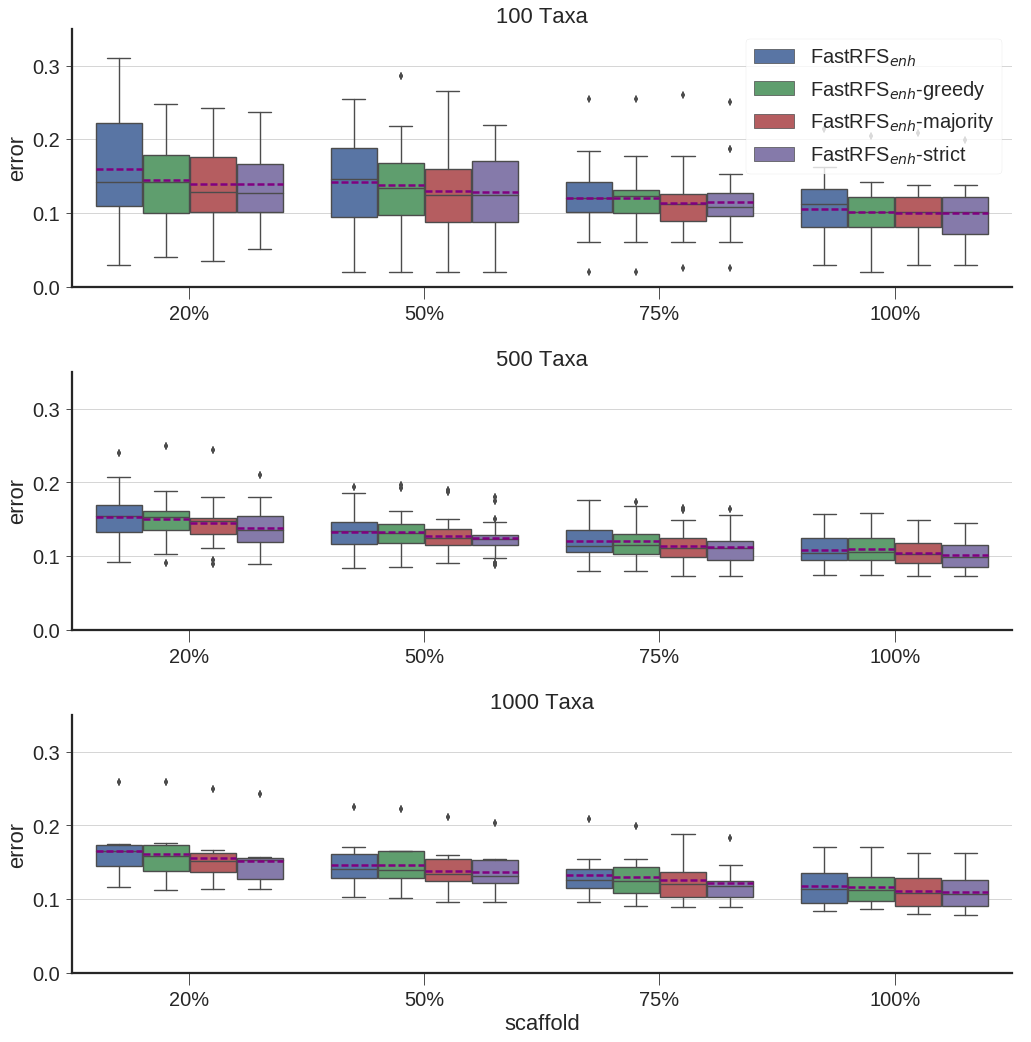
\includegraphics[width=\textwidth]{siesta-supp-figs/fastrfs-enh-consensus-comparison-mult_only}
  \caption[Comparison of  average of FP and FN error rates for  a single FastRFS$_{enh}$ tree as well as the three consensus trees on simulated unrooted supertree datasets]{Comparison of  average of FP and FN error rates for  a single FastRFS$_{enh}$ tree as well as the three consensus trees computed on the optimal FastRFS$_{enh}$ trees on simulated
    unrooted supertree datasets. We show the mean number of optimal
    trees averaged over 25 replicates for 100 and 500 taxa, and 10
    replicates for 1000 taxa.}
  \label{fig:supertree-consensus-comparison-1}
\end{figure}
%Correct Figure 1



\begin{figure}
  \centering
  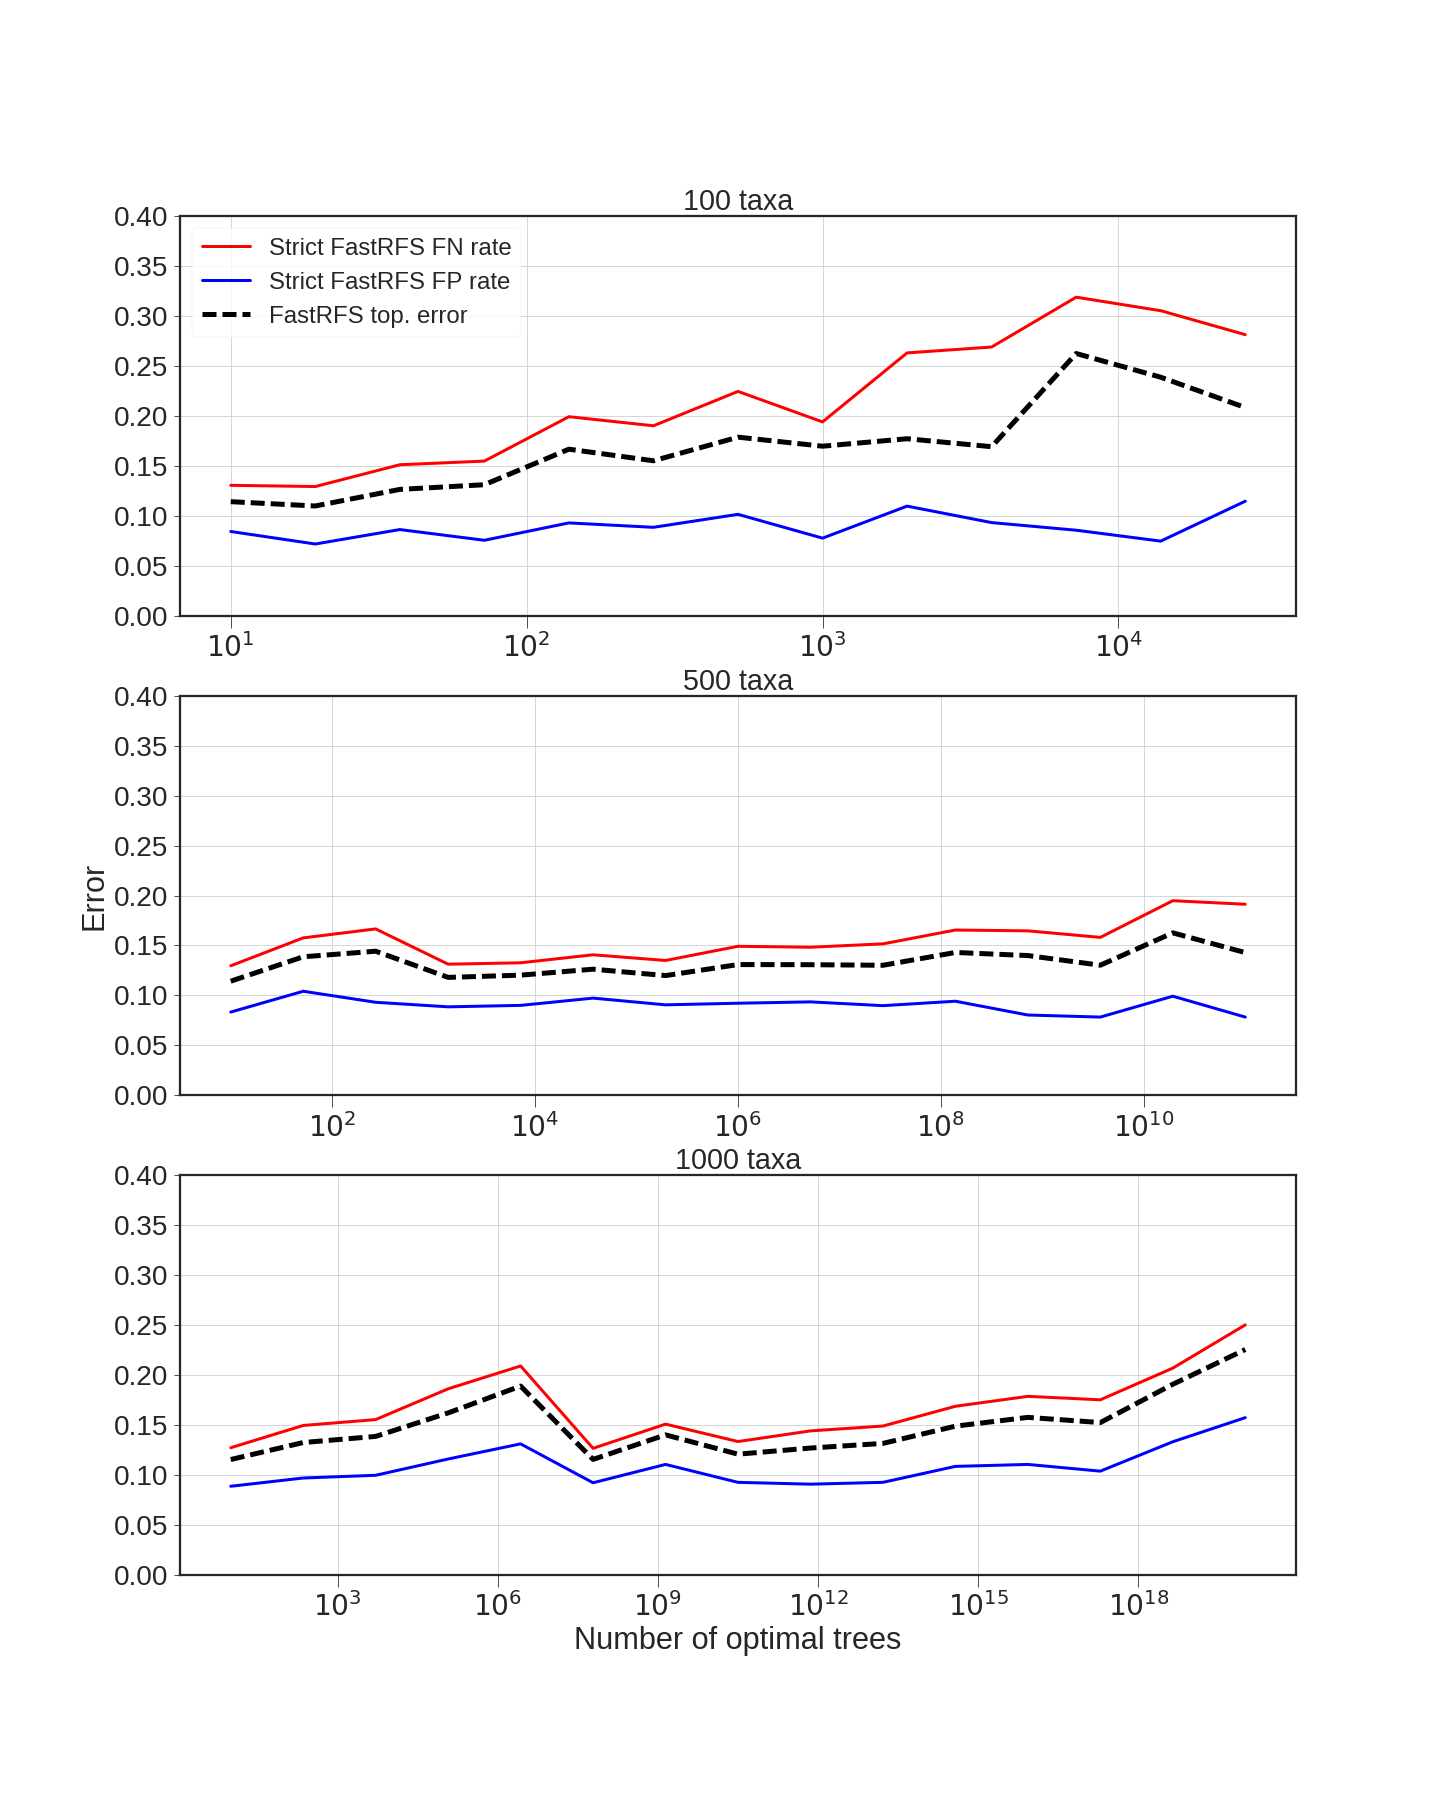
\includegraphics[width=0.9\textwidth]{siesta-supp-figs/fastrfs_ntrees_vs_err}
  \caption[FP and FN rates for FastRFS$_{enh}$ on  simulated unrooted
    supertree datasets as a function of the number of optimal
    trees]{FP and FN rates for FastRFS$_{enh}$ on  simulated unrooted
    supertree datasets as a function of the number of optimal
    trees. Data gathered from 25 replicates for 100 and 500 taxa, and
    10 replicates for 1000 taxa. Red curves show false negative rates;
    blue curves show false positive rates.}
  \label{fig:supertree-consensus-comparison-2}
\end{figure}
%Correct Figure 2


%\clearpage
%\subsection{Rooted Supertree Data Error Rates}




\begin{figure}
  \centering
  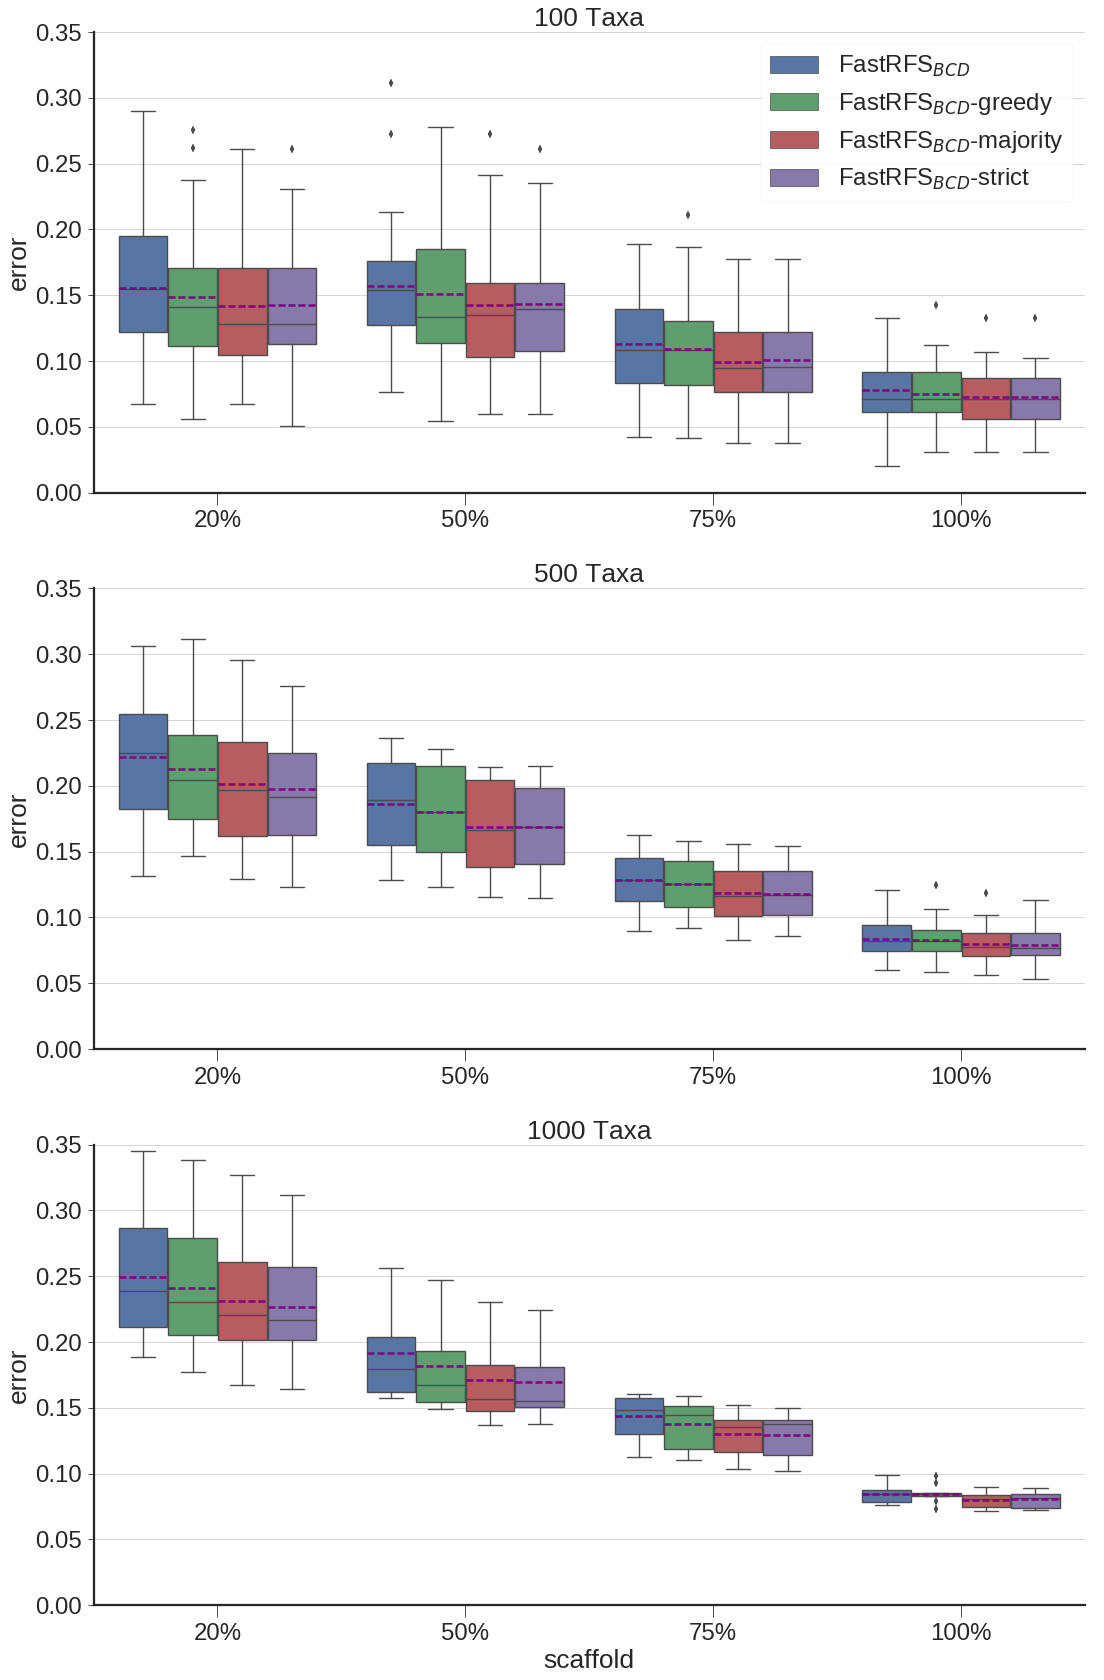
\includegraphics[width=0.9\textwidth,height=0.8\textheight, keepaspectratio]{siesta-supp-figs/fastrfs-bcd-consensus-comparison-mult_only}
  \caption[Comparison of  average FP and FN error rates for a single best FastRFS$_{BCD}$ tree and three  consensus trees  on simulated
    rooted supertree datasets.]{Comparison of  average FP and FN error rates for a single best FastRFS$_{BCD}$ tree and three  consensus trees of the best FastRFS$_{BCD}$ trees  on simulated
    rooted supertree datasets. We show the mean error averaged over 25
    replicates for 100 and 500 taxa, and 10 replicates for 1000 taxa.}
  \label{fig:supertree-consensus-comparison-3}
\end{figure}
%Should be Figure 3



\begin{figure}
  \centering
  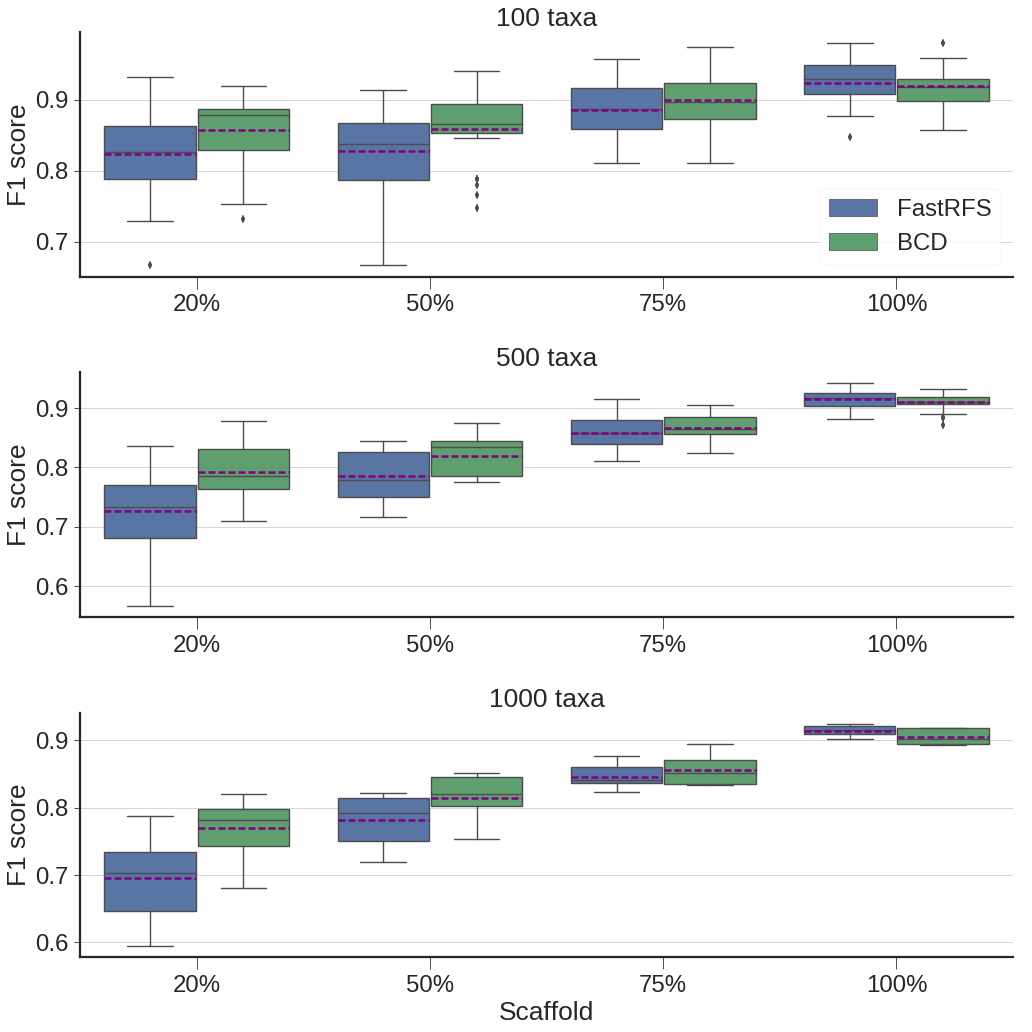
\includegraphics[width=\textwidth]{siesta-supp-figs/fastrfs_basic_smidgenOG_f1}
  \caption[Comparison of F1 scores for a single best FastRFS-basic tree
    and BCD on simulated rooted supertree datasets.]{Comparison of F1 scores for a single best FastRFS-basic tree
    and BCD on simulated rooted supertree datasets. We show the mean
    scores averaged over 25 replicates for 100 and 500 taxa, and 10
    replicates for 1000 taxa.}
  \label{fig:supertree-consensus-comparison-4}
\end{figure}
%Should be Figure 4

\begin{figure}
  \centering
  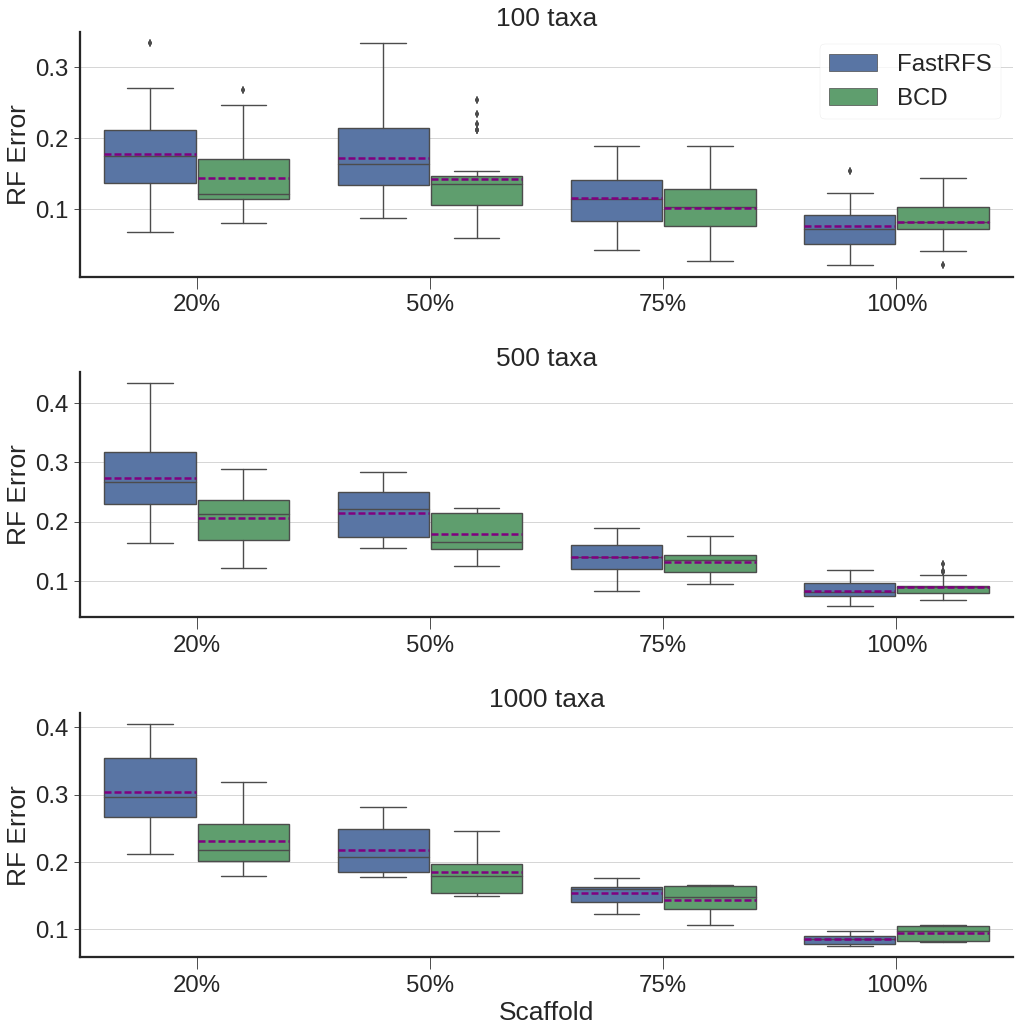
\includegraphics[width=\textwidth]{siesta-supp-figs/fastrfs_basic_smidgenOG_error}
  \caption[Comparison of average RF error rates for a single best FastRFS-basic tree
    and BCD on simulated rooted supertree datasets.]{Comparison of average RF error rates for a single best FastRFS-basic tree
    and BCD on simulated rooted supertree datasets. We show the mean
    error averaged over 25 replicates for 100 and 500 taxa, and 10
    replicates for 1000 taxa.}
  \label{fig:supertree-consensus-comparison-5}
\end{figure}
%Should be Figure 5
\clearpage

\begin{figure}
  \centering
  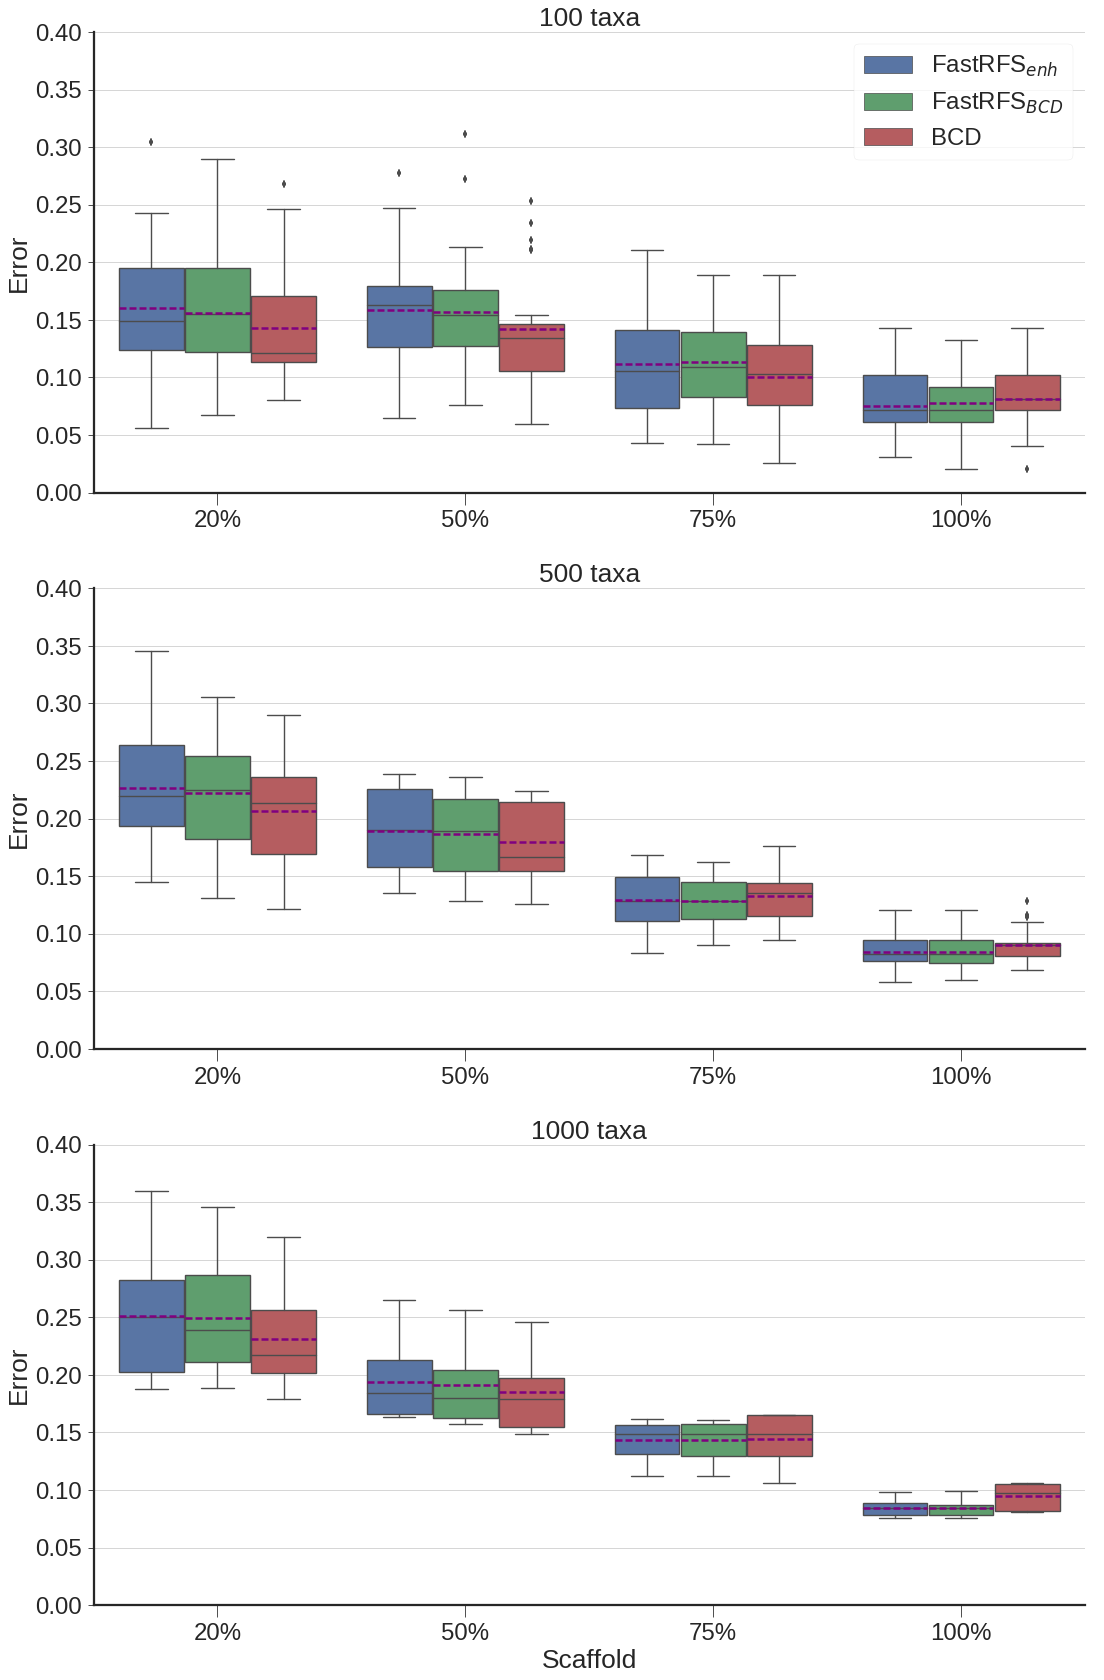
\includegraphics[width=0.9\textwidth,height=0.8\textheight,keepaspectratio]{siesta-supp-figs/fastrfs_nosiesta_smidgenOG_error}
  \caption[Comparison of average RF error rates for  BCD and the single best trees for FastRFS$_{BCD}$ and FastRFS$_{enh}$ on simulated
    rooted supertree datasets.]{Comparison of average RF error rates for  BCD and the single best trees for FastRFS$_{BCD}$ and FastRFS$_{enh}$ on simulated
    rooted supertree datasets. We show the mean error
    averaged over 25 replicates for 100 and 500 taxa, and 10
    replicates for 1000 taxa.}
  \label{fig:supertree-consensus-comparison-6}
\end{figure}
%Should be Figure 6



\begin{figure}
  \centering
  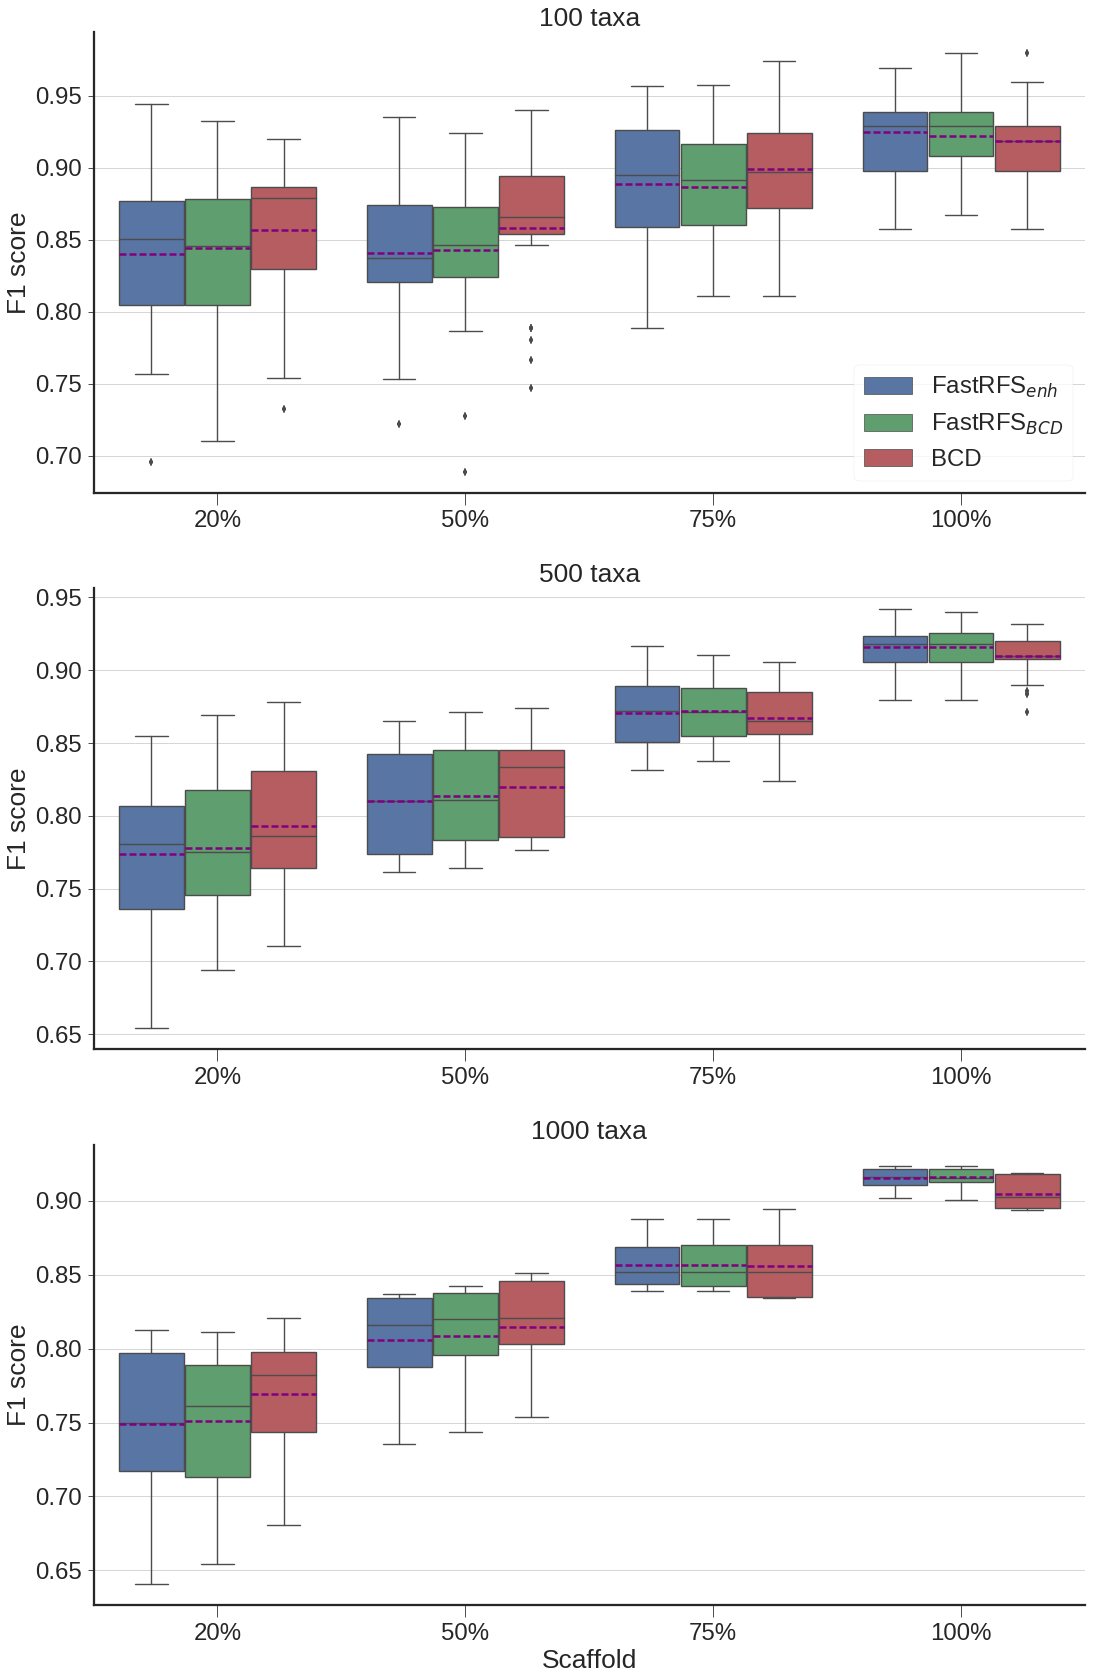
\includegraphics[width=0.9\textwidth,height=0.8\textheight,keepaspectratio]{siesta-supp-figs/fastrfs_nosiesta_smidgenOG_f1}
  \caption[Comparison of F1 scores for  BCD and the single best trees for FastRFS$_{BCD}$ and FastRFS$_{enh}$ on simulated
    rooted supertree datasets.]{Comparison of F1 scores for  BCD and the single best trees for FastRFS$_{BCD}$ and FastRFS$_{enh}$ on simulated
    rooted supertree datasets. We show the mean F1 score
    averaged over 25 replicates for 100 and 500 taxa, and 10
    replicates for 1000 taxa.}
  \label{fig:supertree-consensus-comparison-7}
\end{figure}
%Should be Figure 7




\begin{figure}
  \centering
  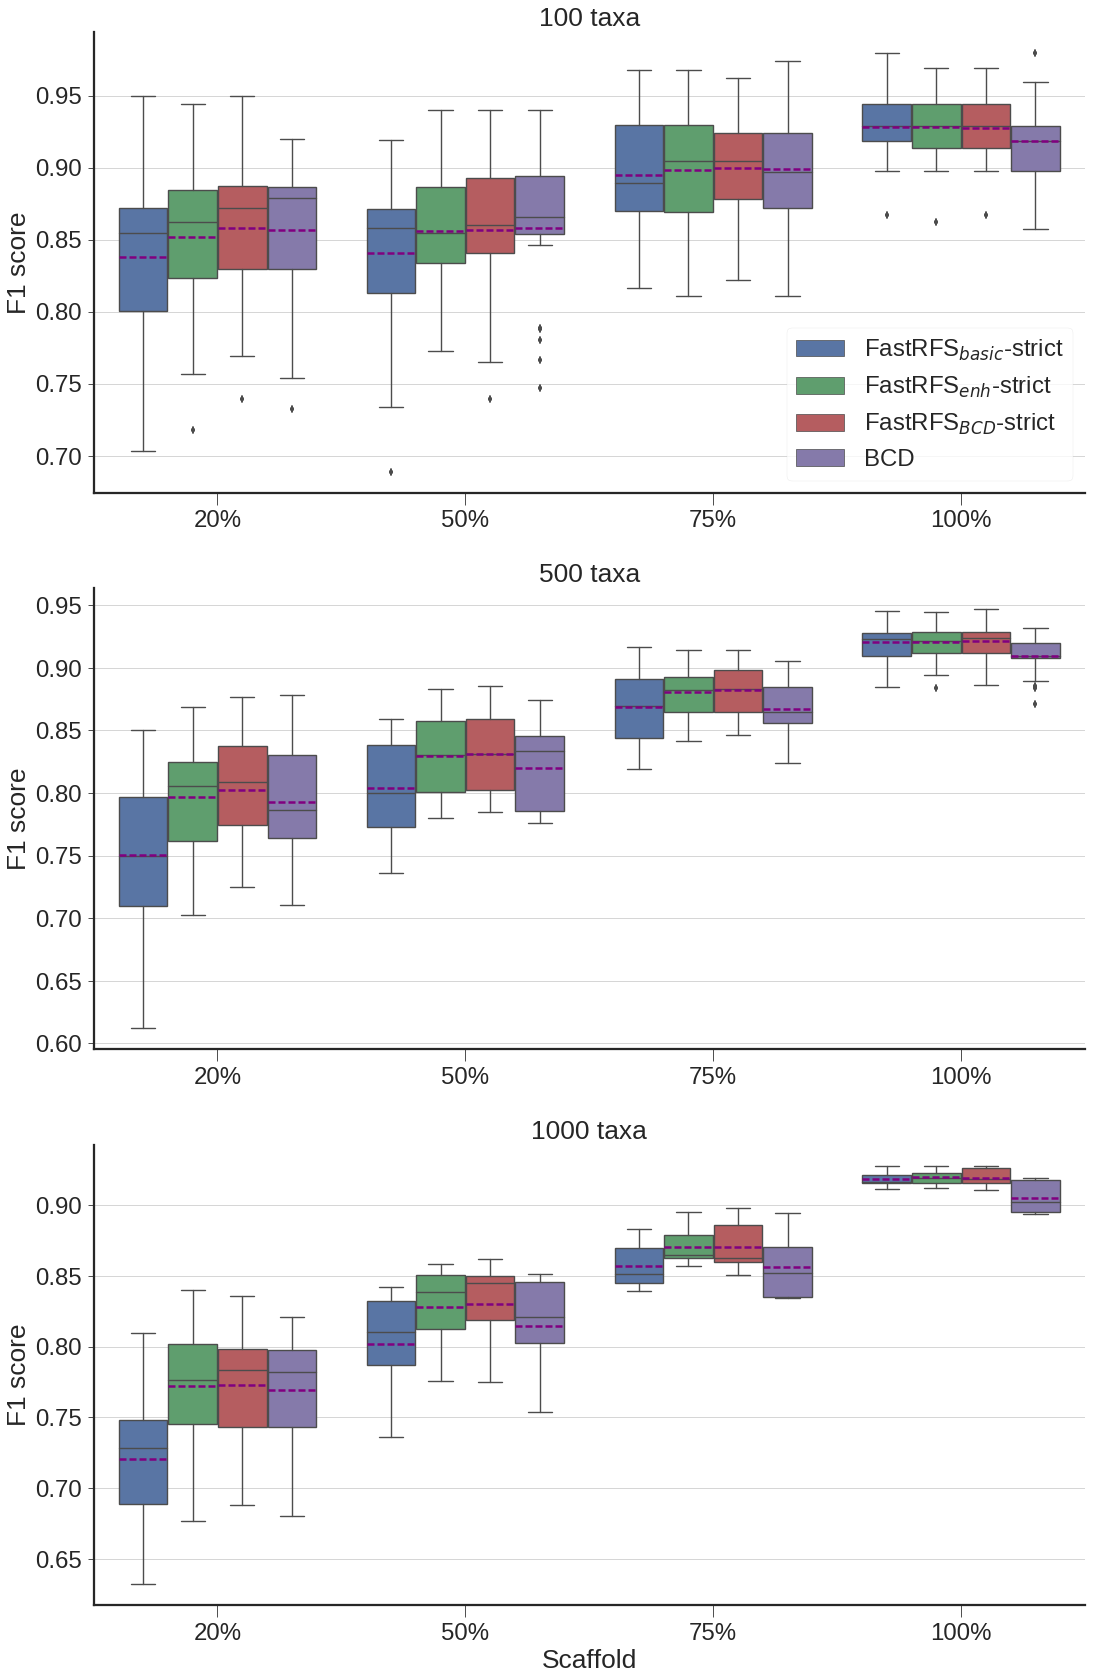
\includegraphics[width=0.9\textwidth,height=0.8\textheight,keepaspectratio]{siesta-supp-figs/fastrfs_smidgenOG_f1}
  \caption[F1 scores for the strict consensus of the optimal FastRFS$_{BCD}$  trees and BCD on
    simulated rooted supertree datasets.]{Comparison of F1 scores for the strict consensus of the optimal FastRFS$_{BCD}$  trees and BCD on
    simulated rooted supertree datasets. We show the mean scores averaged over
    25 replicates for 100 and 500 taxa, and 10 replicates for 1000
    taxa.
    }
  \label{fig:supertree-consensus-comparison-8}
\end{figure}
%Should be Figure 8, but needs to be restricted to just these two methods


%\subsection{Phylogenomic Data Error Rates}

\begin{figure}
  \centering
  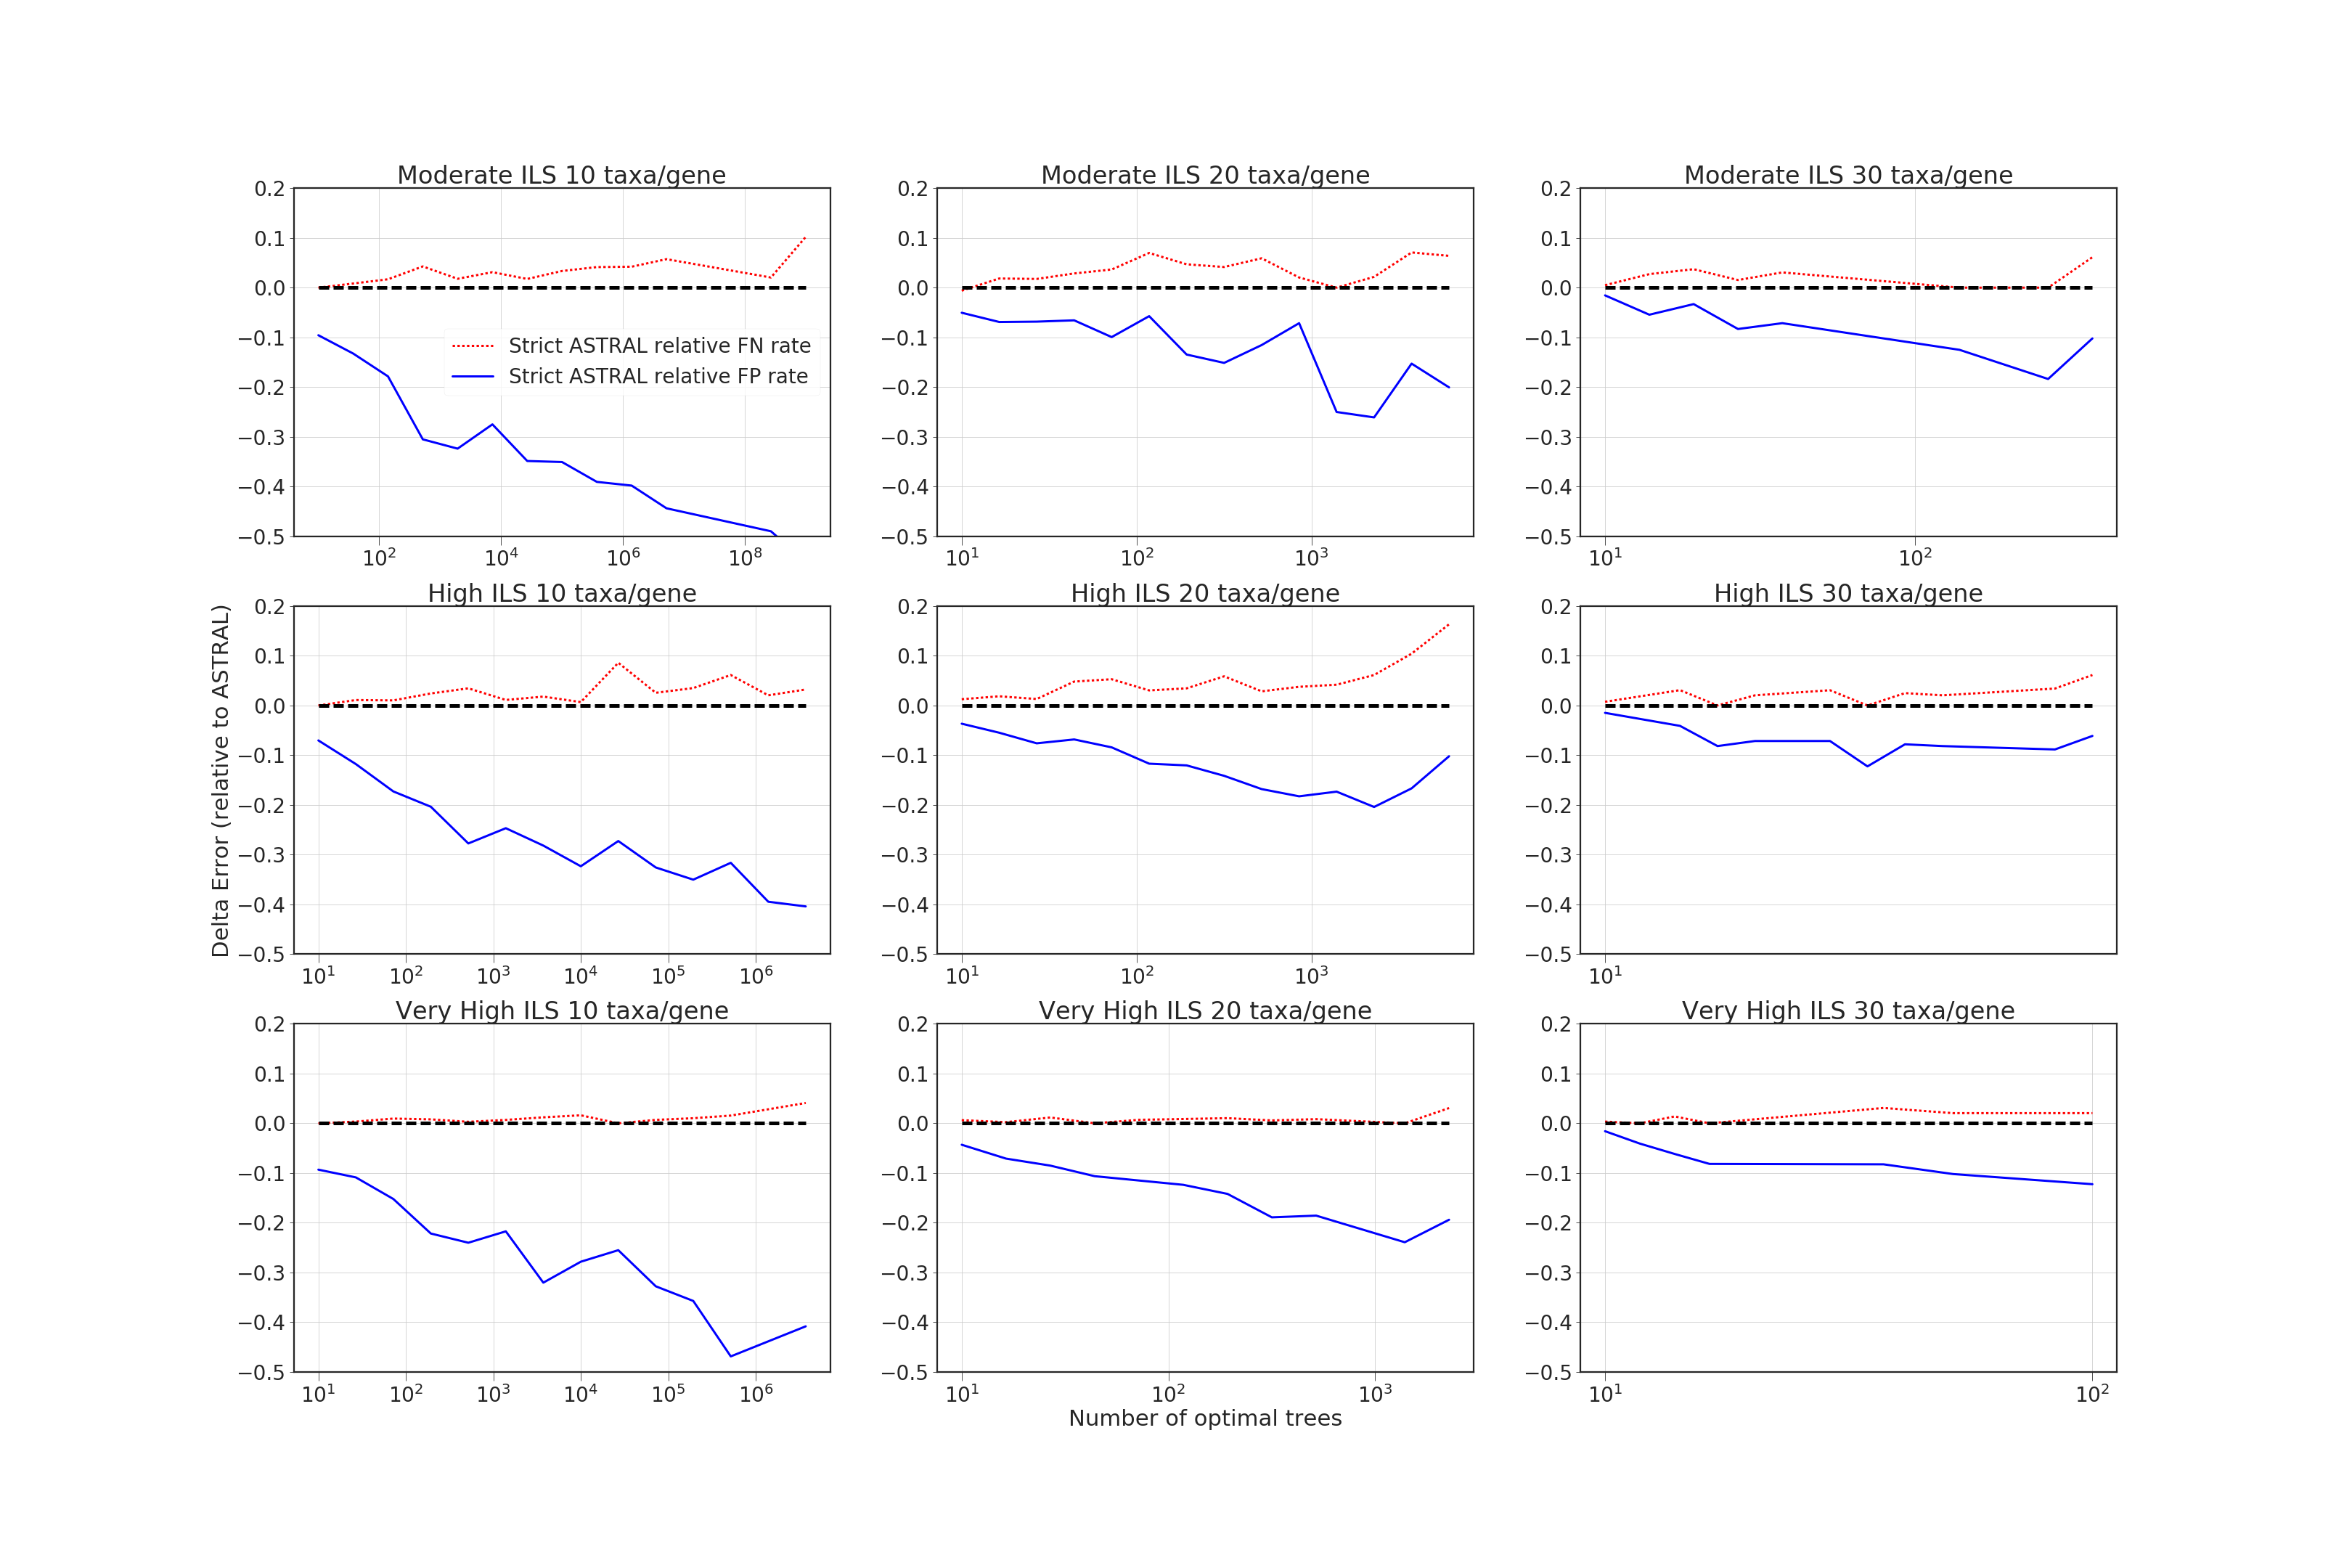
\includegraphics[width=\textwidth]{siesta-supp-figs/astral_missing_ntrees_vs_err.png}
  \caption[Change in FP and FN rates for  the strict consensus of the optimal ASTRAL trees, compared to a single optimal tree, on simulated phylogenomic datasets as a
    function of the number of optimal trees.]{Change in FP and FN rates for  the strict consensus of the optimal ASTRAL trees, compared to a single optimal tree, on simulated phylogenomic datasets as a
    function of the number of optimal trees. Positive values indicate that the strict consensus has a higher error than a single best tree, and negative values indicate that the
    strict consensus has a lower error than a single best tree.  Data  are gathered from 25
    replicates per model condition. Red curves show false negative rates;
    blue curves show false positive rates.}
  \label{fig:supertree-consensus-comparison-9}
\end{figure}
%Should be Figure 9
